% SPDX-License-Identifier: Apache-2.0
\subsection{A narrow prospective deployment region}
The final diagnostic completes 1,920 paired worlds. B adopts in 398, all under the seed-inclusive funding policy:
199 full-history and 199 adoption-only. No earned-funded path adopts.
Four of 160 conditions have positive mean B profit. Every one uses zero integration cost,
.5 arrival probability and adoption-only seed funding: the \money{10}/\money{20} targets under
deterministic/logit choice. Their mean profits are respectively \money{129.51},
\money{106.46}, \money{96.72} and \money{183.28}. No \money{10}-integration or .25-arrival
condition has positive mean B profit.

Twenty conditions have positive mean B-minus-A outcome, all adoption-only seed-funded;
fifteen have a positive lower conditional Monte Carlo bound. Across individual worlds, 82 B paths
are profitable: 66 adoption-only seed, 14 adoption-only earned with no adoption, and two
full-history seed paths. The two individually profitable full-history paths still perform worse
than their A counterparts. Across the diagnostic, 62 B worlds combine positive profit with positive incremental value,
all adoption-only seed-inclusive. Seventy-two direct-payback worlds nevertheless have negative
B-minus-A value. These counts do not estimate a real enterprise's success probability. No full-history condition has positive mean B profit or positive mean B-minus-A effect.

\begin{table}[H]
\centering\small
\caption{Preselected diagnostic slice: \money{20} target, zero integration, .5 work arrival,
ten assumed avoided minutes, logit, twelve reused seeds. A mean profit is \money{-1.69}
in all rows. Monetary values are simulated USD.}
\begin{tabularx}{\textwidth}{Yrrrr}
\toprule
Cost and funding basis & B mean profit & B--A mean & Adopted & Profitable\\
\midrule
Full history; earned & $-363.21$ & $-361.52$ & 0/12 & 0/12\\
Adoption only; earned & $-1.69$ & $0.00$ & 0/12 & 4/12\\
Full history; seed & $-178.24$ & $-176.55$ & 12/12 & 1/12\\
Adoption only; seed & $183.28$ & $184.97$ & 12/12 & 12/12\\
\bottomrule
\end{tabularx}
\end{table}

Prospective B profit ranges from \money{15.03} to \money{397.09}, with median
\money{122.65} and sample standard deviation \money{119.69}. Paired gains range
\money{62.31}--\money{314.62}, median \money{158.36}, standard deviation \money{78.06}.
With historical cost included, 11/12 B paths lose money: the range is
\money{-346.49}--\money{35.57}, median \money{-238.87}. Every paired investment effect
is negative in that full-history condition, from \money{-299.21} to \money{-46.90}.
These are realized model dispersions, not uncertainty bounds on real markets.

In the last row the mean-profit interval is [\money{115.56}, \money{251.00}], and the paired
increment interval is [\money{140.80}, \money{229.13}]. All twelve paths directly repay the
prospective adoption and upkeep. The \money{20} quote remains \money{20} before and after
adoption, so this slice does not depend on a hidden automatic price reduction.
At the \money{10} target, actual quotes fall from the \money{14.33} cost floor to \money{10}
after adoption; that channel is explicitly recorded.

\begin{figure}[H]
\centering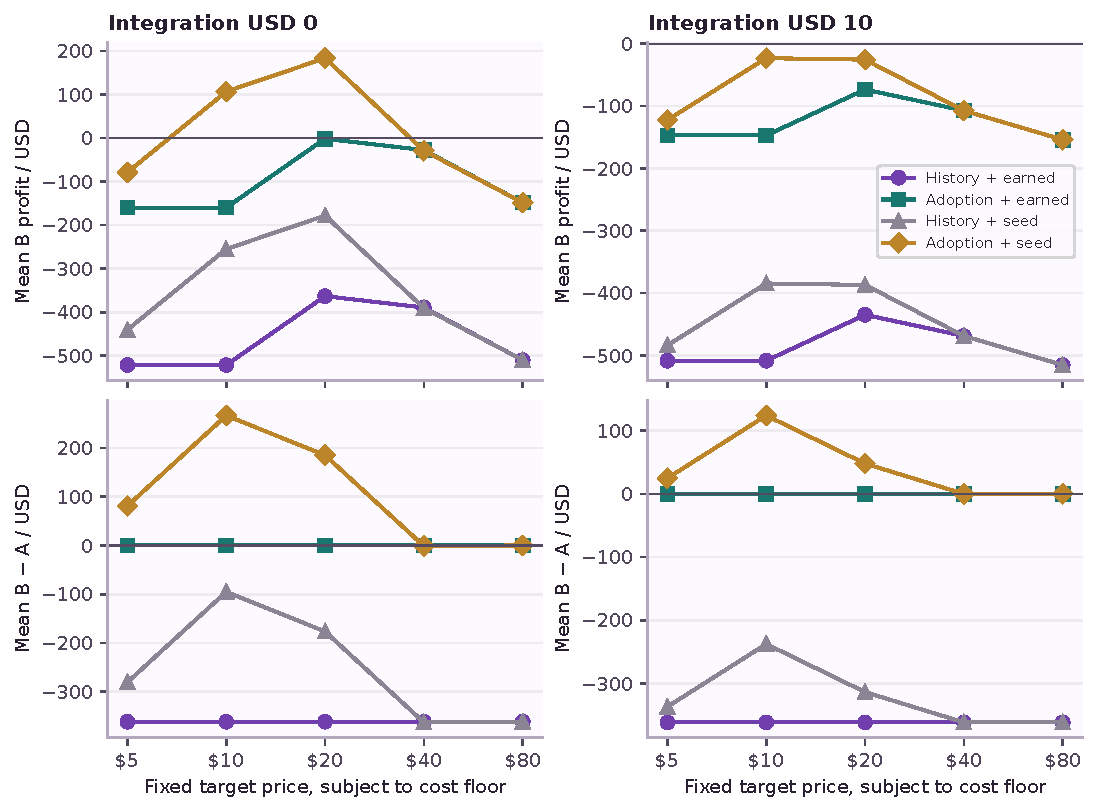
\includegraphics[width=\textwidth]{figures/policy.pdf}
\caption{All five target policies in the predeclared figure slice, including losing prices.
Top: mean B economic profit. Bottom: paired B-minus-A effect. Arrival .5, ten assumed avoided
minutes and logit are fixed. Adding \money{10} integration eliminates positive mean profit.
Full-history and prospective accounting are never pooled. Exact intervals and all 160
configurations appear in the companion table.}
\end{figure}

\subsection{One connected enterprise history}
The preselected seed 2001 illustrates deployment without selecting a winning trajectory after
the run. Under adoption-only seed funding it has 282 new-work opportunities, of which 213 fit
scope. The enterprise attempts 29, accepts 28 and rejects one; alternatives and deferral handle
the rest. At week 8, \money{745.37} is currently available after obligations and reserve.
The exact producer's \money{32.69} prospective adoption charge fits that cash, service pauses
one week and the asset becomes available at week 9. It is used on 17 subsequent modeled jobs.

The same enterprise collects \money{560}, incurs \money{437.35} total declared prospective
costs including a \money{20} refund, and finishes with \money{122.65} profit and
\money{1,122.65} cash. Adoption plus upkeep is \money{54.19}; direct avoided cost is
\money{190.75}. Its paired incremental gain is \money{136.56}. The AI competitor responds with
lower quotes and pays \money{200} for its declared automation at week 12. All these events are
simulated; the source-bound packet remains the actual production evidence.

The earned-surplus gate still reports \money{-77.35}, because this financing rule withholds a
\money{200} reserve from accumulated net earnings as well as checking liquidity.
Available cash and earned funding are deliberately different. The same path including
historical research finishes at \money{-238.87} profit and \money{-224.96} incremental value.
A visible cash balance therefore cannot be presented as historical cost repayment. Sixteen
other diagnostic paths end with positive earned availability after the reserve, but none has
a second constructed and tested asset to purchase.

\begin{figure}[H]
\centering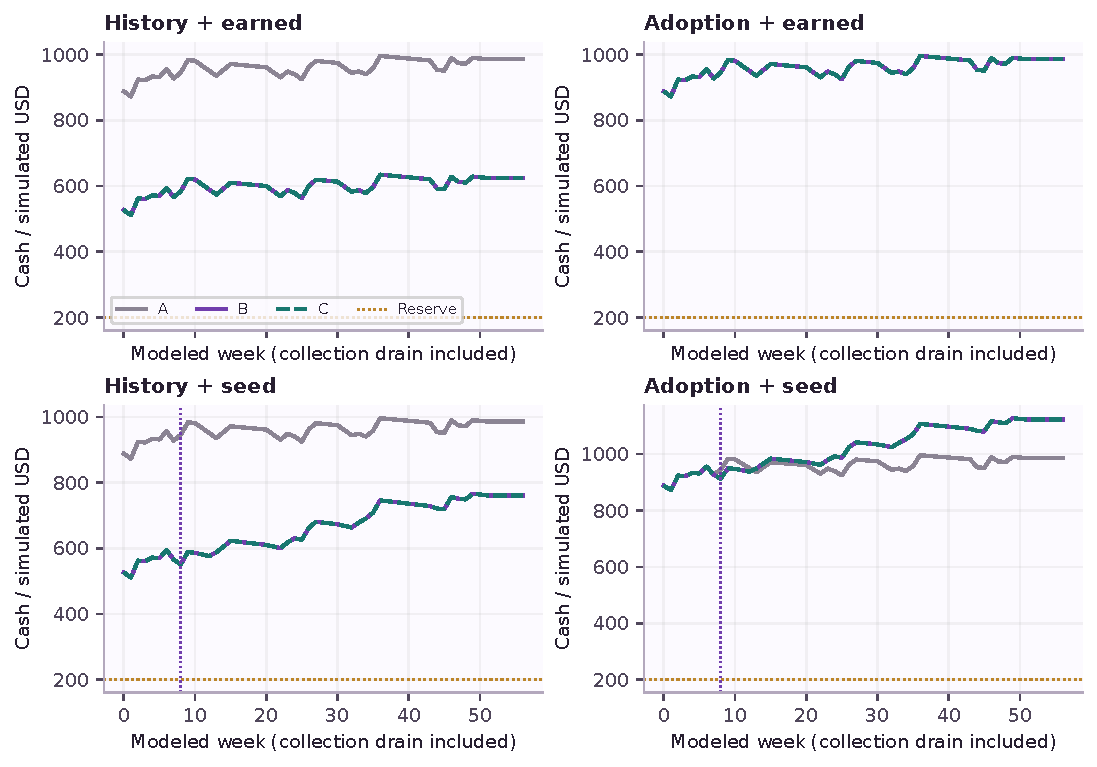
\includegraphics[width=\textwidth]{figures/history.pdf}
\caption{The same preselected seed across four accounting/funding regimes. B and C overlap.
Dotted vertical lines mark adoption; the horizontal line is the liquidity reserve.
Final collection weeks remain in the trace. No later hypothetical asset is purchased.}
\end{figure}

The narrow prospective region is a post-exploratory diagnostic on reused seeds. At this stage,
it has not been independently confirmed or stress-validated under every fixed-price interaction.
The earlier cheap-competitor, maintenance and quality stresses remain preserved, but their
heuristic-price outcomes cannot certify robustness of these new target policies.
A separately frozen fresh-seed extension follows below. It probes robustness of this selected
policy without identifying an optimal price or outside-market predictive performance.
